\chapter{Zybo}

\section{Zynq}
\subsection{Übersicht}
Der Zynq-7000 ist ein SoC\footnote{System on Chip} der einen 667 MHz Dual-Core ARM Cortex-A9 Prozessor und einem programmierbare Logik enthält, die einem Artix-7 FPGA entspricht.
Der Prozessor und dessen Peripherie befindet sich im \textit{Processing System} oder kurz PS.
Der FPGA-Teil des Zynq wird oft PL oder \textit{Programmable Logic} genannt.
Über den AMBA-Bus kann der Prozessor und auch die PL auf die Peripherie, wie z.B. SPI, GPIO, Ethernet oder auch DDR3 zugreifen.
Das Block Diagramm in der Abbildung \ref{fig:BlockDiagrammZynq} gibt einen guten Überblick über den ganzen SoC.

\begin{figure}[htbp]
	\centering
		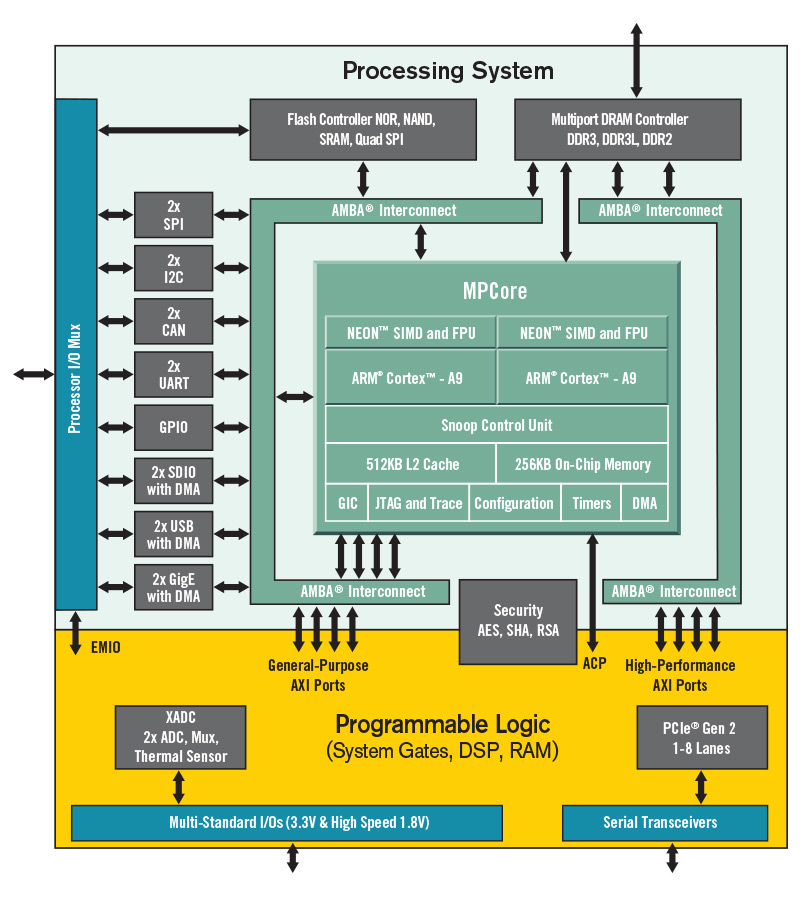
\includegraphics[width=10cm,height=\textheight,keepaspectratio]{images/zynqBlockDiagram.png}
	\caption[Block Diagramm Zynq\-7000]{Block Diagramm Zynq\-7000\footnotemark}
	\label{fig:BlockDiagrammZynq}
\end{figure}
\footnotetext{https://www.xilinx.com/products/silicon-devices/soc/zynq-7000.html}


\subsection{MIO und EMIO}
MIOs sind \textit{Multiplexed Input Output Pins} welche direkt vom Prozessor angesprochen werden können, ohne dass die PL programmiert werden muss.
Die EMIOs sind \textit{\textbf{Extended} Multiplexed Input Output Pins} welche direkt an die PL angeschlossen sind.
Aus diesem Grund können die EMIOs nur verwendet werden, wen die PL entsprechend programmiert wurde.
Diese Arbeit beschränkt sich nur auf die MIOs und das PS.
Im TRM\footnote{Technical Reference Manual} des Zynq\ref{bib:ZynqTechnicalReferenceManual} im Kapitel \textit{''2.5.4 MIO-at-a-Glance Table''} ist eine sehr gute Übersicht über alle möglichen Funktionen der MIOs gegeben.



\section{Standard Zybo Workflow}
Im \textit{Getting Started with Zynq\footnote{https://reference.digilentinc.com/learn/programmable-logic/tutorials/zybo-getting-started-with-zynq/start?redirect=1}} Tutorial von Digilent ist beschrieben, wie man ein einfaches Design für die PL und ein einfaches Programm für das PS erstellt.
Das Tutorial deckt den ganzen Workflow ab.
Dabei werden, z.B. für LED1 bis LED3, auch die EMIOs verwendet.
In Schritt 1 bis 7 wird mit Vivado das Design für die PL erstellt und exportiert.

\textit{Hinweis1:} Die Zybo Toolchain benötigt den standard USB Treiber. Im Kapitel \ref{kapitel:usbTreiber} ist beschrieben, wie der standard USB Treiber wieder installiert werden kann.

\textit{Hinweis2:} Vivado und die Xilinx SDK müssen für dieses Tutorial installiert sein.

Ab Schritt 8 wird beschrieben, wie im XSDK (\textit{Xilinx Standard Development Kit}) ein einfaches ''Hello World'' Programm in C für den Prozessor geschrieben werden kann.
% Das XSDK ist Eclipse mit einem Xylinx Plug-In.

Das XDSK verwendet im Hintergrund das XSCT\footnote{https://www.xilinx.com/html\_docs/xilinx2018\_1/SDK\_Doc/xsct/intro/xsct\_introduction.html} (\textit{Xilinx Software Command-Line Tool}).
Das XDSK kann interaktiv, oder mit Scripts verwendet werden.
% Die Scriptsprache basiert, wie auch Jim-TCL, auf der Sprache TCL.
Wie auch Jim-TCL basiert die verwendete Scriptsprache auf der Sprache TCL.
Wird das ''Hello World'' Programm im XSDK gestartet, erhält man im \textit{SDK Log} Fenster ein detailliertes Log des ausgeführten Script.
In diesem Log kann man nachvollziehen, was das Script beim Download und Start des Programmes alles ausgeführt.

% TODO was auch immer
Im Anhang \ref{anhang:SDKLog} ist eine Kopie eines solchen Logs zu finden.
% langesWort
\textit{D:/Vivado/01\_gettingStarted/01\_gettingStarted.sdk/.sdk/launch\_scripts/xilinx\_c-c++\_application\_(system\_debugger)/system\_debugger\_using\_debug\_01\_gettingstarted\_applicationproject.elf\_on\_local.tcl}
% \textit{D:/Vivado\01\_gettingStarted\01\_gettingStarted.sdk\.sdk\launch\_scripts\xilinx\_c-c++\_application\_(system\_debugger)\system\_debugger\_using\_debug\_01\_gettingstarted\_applicationproject.elf\_on\_local.tcl}

Das Script \textit{ps7\_init.tcl} definiert unter anderem die fünf Initialisierungs-Methoden:
\begin{itemize}
%\begin{itemize}
\item \textit{ps7\_mio\_init\_data\_3\_0}
\item \textit{ps7\_pll\_init\_data\_3\_0}
\item \textit{ps7\_clock\_init\_data\_3\_0}
\item \textit{ps7\_ddr\_init\_data\_3\_0}
\item \textit{ps7\_peripherals\_init\_data\_3\_0}
\end{itemize}
Die Initialisierungs-Methoden werden in der Methode \textit{ps7\_init} aufgerufen.
\textit{ps7\_init} wiederum wird in Zeile 8 des \textit{...elf\_on\_local.tcl} Scripts aufgerufen, welches beim Start des ''Hello World'' Programm im XSDK ausgeführt wird.
In Zeile 9 vom \textit{...elf\_on\_local.tcl} wird auch noch die Methode \textit{ps7\_post\_config} von \textit{ps7\_init.tcl} auf, welche im Anschluss \textit{ps7\_post\_config\_3\_0} aufruft.

Alle Methoden sind auf den folgenden vier Grundbefehlen aufgebaut:\\
% \begin{itemize}
% \item \textit{mwr -force <address> <value>: }         Schreibt den Wert <value> in die Adresse <address>.
% \item \textit{mask\_write <address> <mask> <value>: } Schreibt die Bits der Maske <mask> von <value> in die Addresse <address>.
% \item \textit{mask\_poll <address> <mask>:  }         Wartet bis die maskierten Bits <mask> des Speicherinhalt von der Speicheradresse <mask> gleich 0 sind.
% \item \textit{mask\_dellay <address> <value>:}        Wartet <value> Millisekunden.
% \end{itemize}


\textbf{mwr -force <address> <value>: }\\
Schreibt den Wert <value> in die Adresse <address>.

\textbf{mask\_write <address> <mask> <value>: }\\
Schreibt die Bits der Maske <mask> von <value> in die Addresse <address>.

\textbf{mask\_poll <address> <mask>:  }\\
Wartet bis die maskierten Bits <mask> des Speicherinhalt von der Speicheradresse <mask> gleich 0 sind.

\textbf{mask\_dellay <address> <value>:}\\
Wartet <value> Millisekunden.

% TODO silikon version überprüfen ps7_init.tcl.745


\textbf{ps7\_mio\_init\_data\_3\_0:}\\
Diese Methode initialisiert die MIOs.
Es wird der Multiplexer für die IO Pins konfiguriert.
Dadurch wird definiert, welcher Pin von welcher Peripherie, wie UART und auch RAM, verwendet wird.
Zusätzlich werden auch, falls vorhanden, folgende elektrischen Charakteristiken definiert:
\begin{itemize}
\item \textbf{PULLUP:} Pullup Widerstand aktivieren / deaktivieren.
\item \textbf{IO\_Type:} Buffer Type: LVCMOS 1.8V, LVCMOS 2.5V, LVCMOS 3.3V,  oder HSTL.
\item \textbf{SPEED:} Slow oder Fast CMOS edge.
\item \textbf{Tristate:} Enalbe / disable Tristate.
\end{itemize} 


\textbf{ps7\_pll\_init\_data\_3\_0}\\
Initialisiert die drei PLLs\footnote{Phase Locked Loop} ARM, DDR und IO.
Bei jeder PLL-Initialisierung wird darauf gewartet, bis der PLL betriebsbereit (locked) ist.
Die Dauer dieser Wartezeit ist unbekannt.

\textbf{ps7\_clock\_init\_data\_3\_0}\\
Konfiguriert diverse Clocks, die im Prozessor gebraucht werden.

\textbf{ps7\_ddr\_init\_data\_3\_0}\\
Konfiguriert den DDR Bus.
Für die Konfiguration werden insgesamt 79 verschiedene Register geschrieben und die DCI (Digital Controlled Impedance) kalibriert.

\textbf{ps7\_peripherals\_init\_data\_3\_0}\\
Konfiguriert folgende Peripherie:
\begin{itemize}
\item UART1
\item QSPI (für Flash Speicher auf Zybo)
\item POR timer
\item High-Low-Wait(1msec)-High Sequenz für MIO46 (USB-OTG Ping)
\end{itemize} 




Die oben genannten Initialisierungsfunktionen werden vom Xilinx Debugger jedes mal ausgeführt, wenn die Applikation im XSDK mit \textit{''Launch on Hardware (System Debuger)''} gestartet wird.
Es ist aber auch möglich, die Initialisierung direkt mit der C-Applikation und nicht mit dem Debugger durchzuführen.
Wird die Initialisierung in der Applikation durchgeführt, und die Applikation auf dem Flash Speicher des Zynq gespeichert, dann Initialisiert sich der Zynq bei jedem Start selber.
Im Beispielprogramm \textit{''helloworld.c''} ist die Methode \textit{''init\_platform()''} enthalten, welche in \textit{''platform.c''} deklariert ist.
Standardmässig ist sie aber auskommentiert.
\textit{''platform.c''} befindet sich im \textit{''design\_wrapper\_hw\_platform''} welcher in Vivado erzeugt wurde.
\textit{''ps7\_init()''}


\textit{helloworld.c:}
\lstset{language=c}
\begin{lstlisting}[frame=single]
...
#include "platform.h"
..
int main ()
{
...
init_platform();

while(1){
...
\end{lstlisting}



\textit{platform.c:}
\lstset{language=c}
\begin{lstlisting}[frame=single]
...
/*#include "ps7_init.h"*/
/*#include "psu_init.h"*/
...
void
init_platform()
{
    /*
     * If you want to run this example outside of SDK,
     * uncomment one of the following two lines and also #include "ps7_init.h"
     * or #include "ps7_init.h" at the top, depending on the target.
     * Make sure that the ps7/psu_init.c and ps7/psu_init.h files are included
     * along with this example source files for compilation.
     */
    /* ps7_init();*/
    /* psu_init();*/
    enable_caches();
    init_uart();
}
...

\end{lstlisting}




% Script anpassen

% 